\exercisesheader{}

% 33 - body_measurements_weight_height_inf_ahss

\eoce{\qt{Body measurements, Part IV\label{body_measurements_weight_height_inf_ahss}} 
The scatterplot and least squares summary below show the relationship 
between weight measured in kilograms and height measured in centimeters 
of 507 physically active individuals.

\noindent\begin{minipage}[c]{0.4\textwidth}
\begin{center}
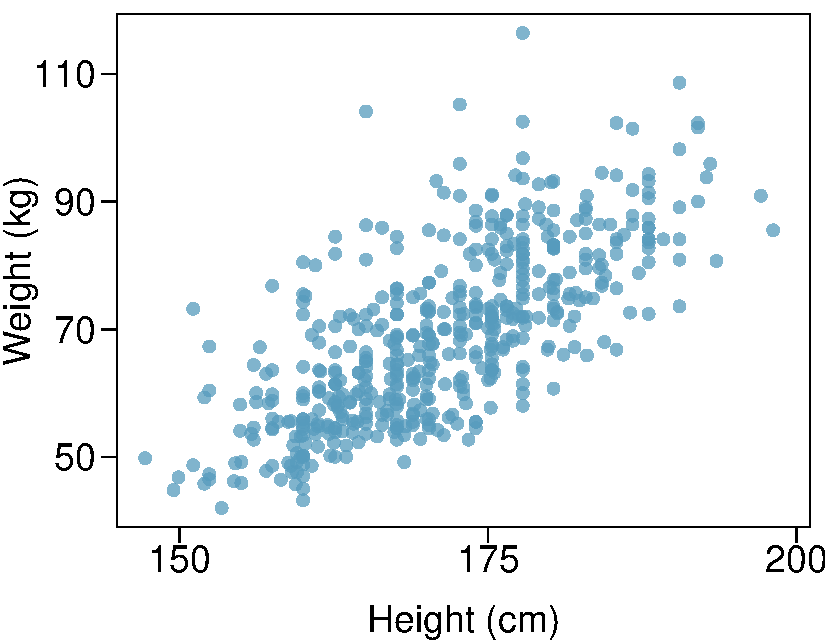
\includegraphics[width=\textwidth]{ch_regr_simple_linear/figures/eoce/body_measurements_weight_height_inf_ahss/body_measurements_weight_height.pdf}
\end{center}
\end{minipage}
\begin{minipage}[c]{0.6\textwidth}
{\scriptsize
\begin{center}
\begin{tabular}{rrrrr}
    \hline
            & Estimate  & Std. Error    & t value   & Pr($>$$|$t$|$) \\ 
    \hline
(Intercept) & -105.0113 & 7.5394        & -13.93    & 0.0000 \\ 
height      & 1.0176    & 0.0440        & 23.13     & 0.0000 \\
    \hline
\end{tabular}
\end{center}
}
\end{minipage}
\begin{parts}
\item Describe the relationship between height and weight.
\item Write the equation of the regression line. Interpret the slope 
and intercept in context.
\item Do the data provide strong evidence that an increase in height 
is associated with an increase in weight? State the null and alternative 
hypotheses, report the p-value, and state your conclusion.
\item The correlation coefficient for height and weight is 0.72. 
Calculate $R^2$ and interpret it in context.
\end{parts}
}{}

% 34 - mcu_box_office_us_predict_ahss

\eoce{\qt{MCU, predict US theater sales\label{mcu_box_office_us_predict_ahss}} 
The Marvel Comic Universe movies were an international movie sensation,
containing 23 movies at the time of this writing.
Here we consider a model predicting an MCU film's gross theater sales
in the US based on the first weekend sales performance in the US.
The data are presented below in both a scatterplot and the model in
a~regression table.
Scientific notation is used below, e.g. 42.5e6 corresponds to
$42.5\times 10^6$.
\begin{center}
\begin{tabular}{rrrrr}
  \hline
  & Estimate & Std. Error & t value & Pr($>$$|$t$|$) \\ 
  \hline
  (Intercept) & 42.5e6 & 26.6e6 & 1.60 & 0.1251 \\ 
  opening\us{}weekend\us{}us & 2.4361 & 0.1739 & 14.01 & 0.0000 \\ 
  \hline
\end{tabular}
\end{center}
\begin{minipage}[c]{0.48\textwidth}
\begin{parts}
\item
  Describe the relationship between gross theater sales in the US and
  first weekend sales in the~US.
\item
  Write the equation of the regression line. Interpret the slope
  and intercept in~context.
\item
  Do the data provide strong evidence that higher opening weekend sale
  is associated with higher gross theater sales? State the null and
  alternative hypotheses, report the p-value, and state your conclusion.
\item
  The correlation coefficient for gross sales and first weekend sales
  is~0.950.
  Calculate $R^2$ and interpret it in~context.
\item
  Suppose we consider a set of all films ever released.
  Do you think the relationship between opening weekend sales
  and total sales would have as strong of a relationship as
  what we see with the MCU~films?
\end{parts}
\vspace{3mm}
\end{minipage}%
\begin{minipage}[c]{0.5\textwidth}
\hspace{0.1\textwidth}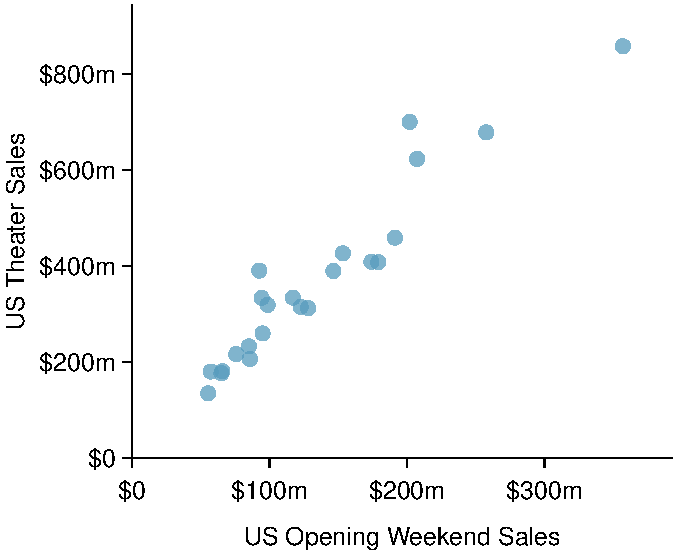
\includegraphics[width=0.9\textwidth]{ch_regr_simple_linear/figures/eoce/mcu_box_office_us_predict_ahss/mcu_box_office_us_predict} \\[3mm]
\end{minipage}
}{}

% 35 - spouses_2_ap

\eoce{\qt{Spouses, Part II\label{spouses_2_ap}} The 
scatterplot below summarizes womens' heights and their spouses' heights for a random 
sample of 170 married women in Britain, where both partners' ages are 
below 65 years. Summary output of the least squares fit for predicting 
spouse's height from the woman's height is also provided in the table.

\noindent\begin{minipage}[c]{0.4\textwidth}
\begin{center}
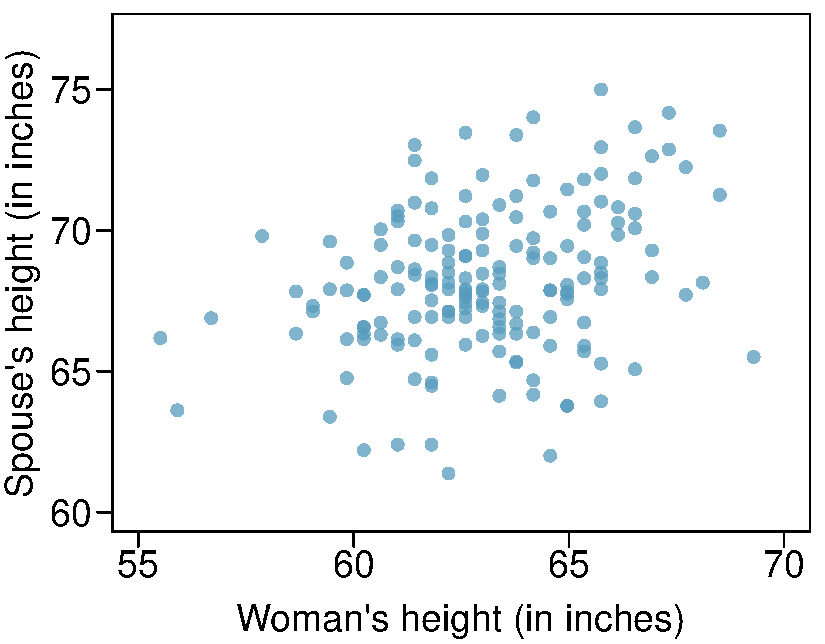
\includegraphics[width=\textwidth]{ch_regr_simple_linear/figures/eoce/spouses_2_ap/husbands_wives_height_inf_2s}
\end{center}
\end{minipage}
\begin{minipage}[c]{0.6\textwidth}
{\scriptsize
\begin{center}
\begin{tabular}{rrrrr}
    \hline
                    & Estimate  & Std. Error    & t value   & Pr($>$$|$t$|$) \\ 
    \hline
(Intercept)         & 43.5755   & 4.6842        & 9.30      & 0.0000 \\ 
height\_\hspace{0.3mm}spouse   & 0.2863    & 0.0686        & 4.17      & 0.0000 \\ 
    \hline
\end{tabular}
\end{center}
}
\end{minipage}
\begin{parts}
\item Is there strong evidence in this sample that taller women have taller spouses? 
State the hypotheses and include any information used to conduct the test.
\item Write the equation of the regression line for predicting the height of a woman's spouse based on the woman's height.
\item Interpret the slope and intercept in the context of the application.
\item Given that $R^2 = 0.09$, what is the correlation of heights 
in this data set?
\item You meet a married woman from Britain who is 5'9" (69 inches). 
What would you predict her spouse's height to be? How reliable is this 
prediction?
\item You meet another married woman from Britain who is 6'7" (79 inches). 
Would it be wise to use the same linear model to predict her spouse's 
height? Why or why not?
\end{parts}
}{}

% 36 - urban_homeowners_cond_ahss

\eoce{\qt{Urban homeowners, Part II\label{urban_homeowners_cond_ahss}}
Exercise~\ref{urban_homeowners_outlier} gives a scatterplot displaying the 
relationship between the percent of families that own their home and 
the percent of the population living in urban areas. Below is a 
similar scatterplot, excluding District of Columbia, as well as the 
residuals plot. There were 51 cases.

\noindent\begin{minipage}[c]{0.45\textwidth}
{\raggedright\begin{parts}
\item For these data, $R^2=0.28$. What is the correlation? How can 
you tell if it is positive or negative?
\item Examine the residual plot. What do you observe? Is a simple 
least squares fit appropriate for these data?
\end{parts}\vspace{15mm}}
\end{minipage}
\begin{minipage}[c]{0.1\textwidth}
$\:$ \\
\end{minipage}
\begin{minipage}[c]{0.43\textwidth}
\begin{center}
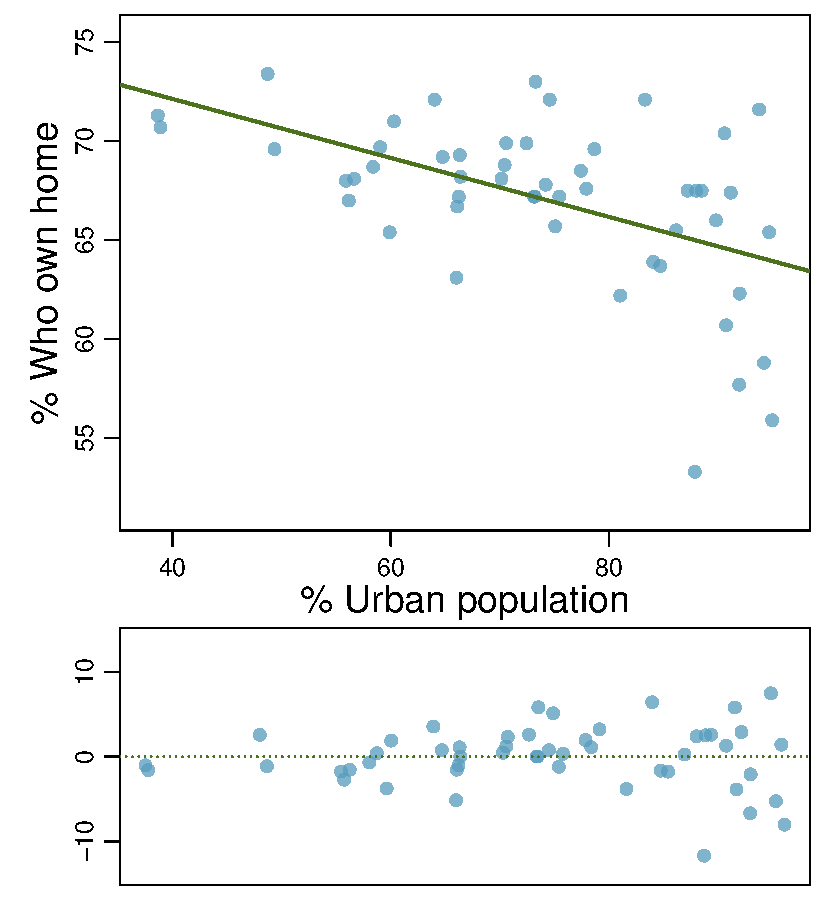
\includegraphics[width=\textwidth]{ch_regr_simple_linear/figures/eoce/urban_homeowners_cond_ahss/urban_homeowners_cond.pdf}
\end{center}
\end{minipage}
}{}

% 37 - murders_poverty_inf_ahss

\eoce{\qt{Murders and poverty, Part II\label{murders_poverty_inf_ahss}} \videosolution{ahss_eoce_sol-murders_poverty_inf} Exercise~\ref{murders_poverty_reg} presents regression output from a model 
for predicting annual murders per million from percentage living in 
poverty based on a random sample of 20 metropolitan areas. The model 
output is also provided below.
\begin{center}
\begin{tabular}{rrrrr}
    \hline
            & Estimate  & Std. Error    & t value   & Pr($>$$|$t$|$) \\ 
    \hline
(Intercept) & -29.901   & 7.789         & -3.839    & 0.001 \\ 
poverty\%   & 2.559     & 0.390         & 6.562     & 0.000 \\ 
    \hline
\end{tabular}
\[ s = 5.512 \qquad R^2 = 70.52\% \qquad R^2_{adj} = 68.89\% \]
\end{center}
\begin{parts}
\item What are the hypotheses for evaluating whether poverty percentage 
is a significant predictor of murder rate?
\item State the conclusion of the hypothesis test from part (a) in 
context of the data.
\item Calculate a 95\% confidence interval for the slope of poverty 
percentage, and interpret it in context of the data.
\item Do your results from the hypothesis test and the confidence 
interval agree? Explain.
\end{parts}
}{}

% 38 - babies_head_gestation_inf

\eoce{\qt{Babies\label{babies_head_gestation_inf}} Is the gestational age 
(time between conception and birth) of a low birth-weight baby useful 
in predicting head circumference at birth? Twenty-five low birth-weight 
babies were studied at a Harvard teaching hospital; the investigators 
calculated the regression of head circumference (measured in centimeters) 
against gestational age (measured in weeks). The estimated regression 
line is
\[ \widehat{head~circumference} = 3.91 + 0.78 \times gestational~age \]
\begin{parts}
\item What is the predicted head circumference for a baby whose 
gestational age is 28 weeks?
\item The standard error for the coefficient of gestational age is 0.
35, which is associated with $df=23$. Does the model provide strong 
evidence that gestational age is significantly associated with head 
circumference?
\end{parts} 
}{}
